%\documentclass[handout, compress,red,mathsans,10pt]{beamer}
\documentclass[compress,red,mathsans,10pt]{beamer}
\usepackage{beamerthemesplit}
\usepackage{amssymb}
%\usetheme{Antibes}
\usepackage{pgf,pgfarrows,pgfnodes}
\usepackage[catalan]{babel}
%\usepackage[latin1]{inputenc}
\usepackage[utf8]{inputenc}

\setbeamercolor{uppercol}{fg=white,bg=purple}%
\setbeamercolor{lowercol}{fg=black,bg=pink}%

%NOTA:
%Per compilar el document:
%
%des de TeXnicCenter: LaTeX=>PS
%des de linea de comandes: ps2pdf nom.ps
%
%

\usecolortheme{lily}
\begin{document}
\title{Aplicacions Estad\'{\i}stiques}
\subtitle{Enginyeria Edificaci\'o 2011/12.}  
\author{Jos\'e Luis Lisani}
\date{}



\frame{\titlepage} 

%\frame{\frametitle{Table of contents}\tableofcontents} 

\section{Presentaci\'o} 
\frame{\frametitle{Informaci\'o general}	
\begin{itemize}
\item Professor: Jos\'e Luis Lisani
\item [] Despatx: Anselm Turmeda D-239
\item [] E-mail: joseluis.lisani@uib.es
\item[] Tutories: dimarts 12h-13h, dimecres 10h30-11h30, dijous 12h-13h
\begin{itemize}
\item[] <2->  \qquad \color{red}concertar cita per email\color{black}
\end{itemize}
\item Horari:
	\begin{center}
	\begin{tabular}{|l|c|} \hline
	D\'{i}a & Hora \\ \hline
	Dimarts & 9:30 -- 11:30 \\ \hline
	Dijous & 9:30 -- 11:30 \\ \hline
	\end{tabular}
	\end{center}
\item Documentaci\'o:
	\begin{itemize}
	\item Campus Extens (apunts, llistes problemes, anuncis)
	\item UIB digital (guia docent, cronograma)
	\item Informaci\'o general estudis: http://enginyeriadedificacio.wordpress.com/
	\end{itemize} 
\end{itemize}
}
\frame{\frametitle{Avaluaci\'o}
\begin{itemize}
\item Activitats presencials: 
	\begin{itemize}
	\item Classes de teoria i problemes 
	\item Examens: 15/03, 03/04, 17/05, \color{red}18/06, (10/09) \color{black}
	\end{itemize}
\item Activitats no presencials: 
	\begin{itemize}
	\item Pràctiques ordinador: 17/04
	\item Entrega de problemes: 03/04, 17/05, 07/06
	\end{itemize}
\item Itineraris:
	\begin{center}
	\begin{tabular}{|l|c|c|c|c|} \hline
			       & A	& B	& C  &  \\ \hline
	Controls peri\`odics    &	& 30\%	& 30\% & No recuperable\\ \hline
	Exercicis              & 20\%	&	& 20\% & No recuperable\\ \hline
	Pr\`actiques ordinador & 10\%	& 10\%	& 10\% & Recuperable\\ \hline
	Examen final           & 70\%	& 60\%	& 40\%  & Recuperable\\ \hline
	\end{tabular}
	\end{center}
\item A l'examen final s'haur\`a de treure una \color{red}nota m\'{\i}nima de 4 \color{black} (sobre 10) per aprovar l'assignatura
\item A cada alumne se li posar\'a la nota \color{red}m\'es favorable dels 3 itineraris \color{black}
\end{itemize}
}

\frame{\frametitle{L'assignatura}
\begin{itemize}
\item Estad\'istica: Ci\`encia per a la descripci\'o, organitzaci\'o i interpretaci\'o de dades
\item <2->Esquema:
\end{itemize}
\begin{columns}
\begin{column}{0.65\textwidth}
\begin{overlayarea}{0.65\textwidth}{0.65\textheight}
 \only<2>{
\includegraphics[width=10cm]{Dbes0101.eps}
		\put(-240,105){Poblaci\'o}
		\put(-260,135){$N$}
	} 
 \only<3>{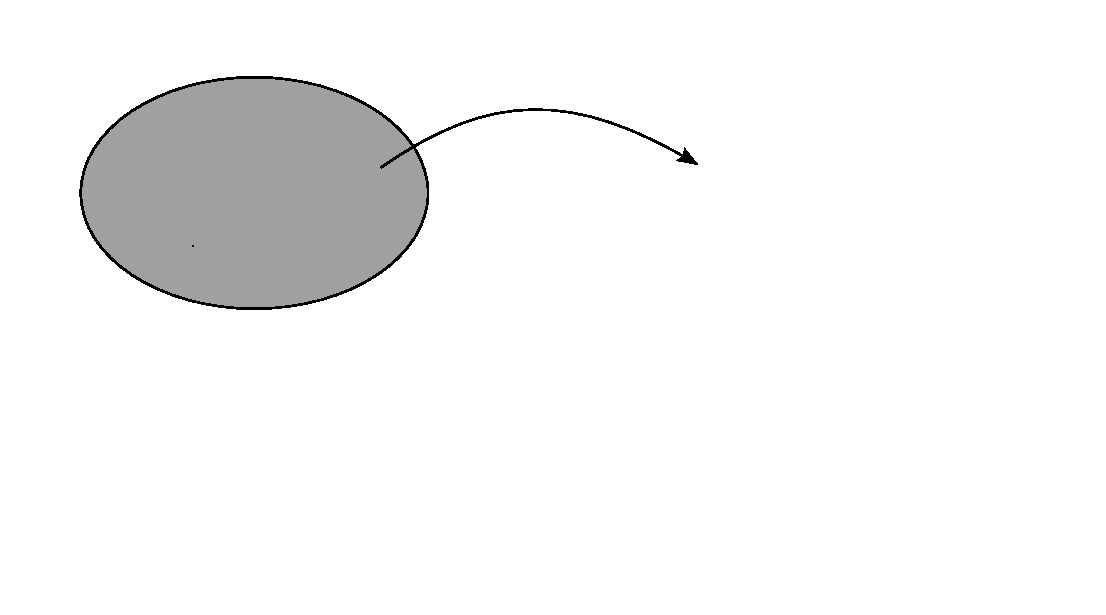
\includegraphics[width=10cm]{Dbes0102.eps}
		\put(-240,105){Poblaci\'o}
		\put(-260,135){$N$}
		\put(-150,135){$X$}
		\put(-110,125){$\mu_{X}, \sigma^2_{X}$}
	} 
 \only<4>{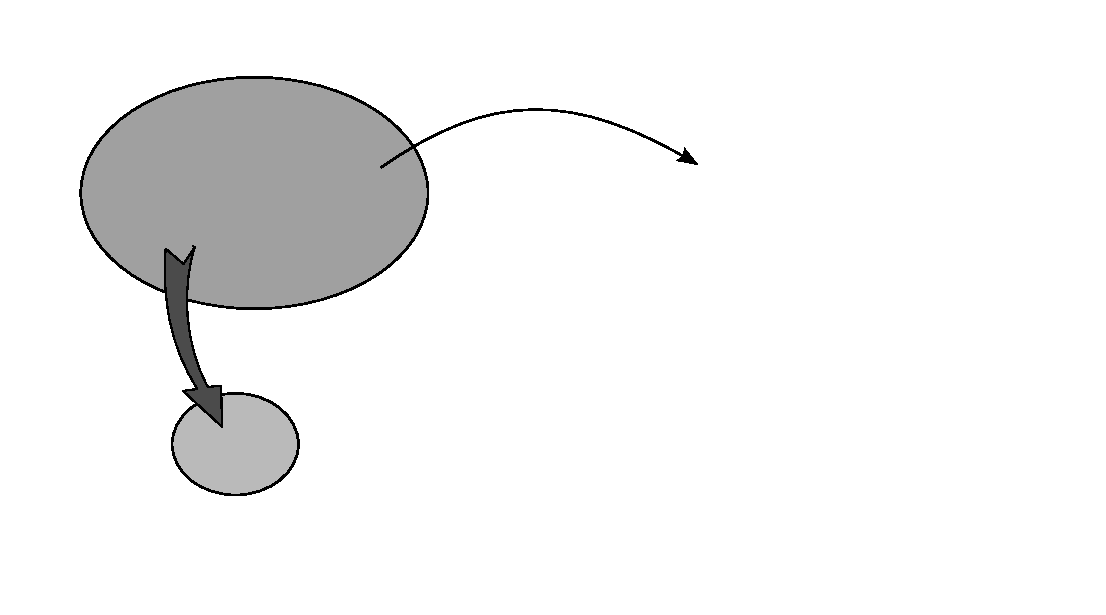
\includegraphics[width=10cm]{Dbes0103.eps}
		\put(-240,105){Poblaci\'o}
		\put(-260,135){$N$}
		\put(-150,135){$X$}
		\put(-110,125){$\mu_{X}, \sigma^2_{X}$}
		\put(-230,65){$n$}
		\put(-240,37){mostra}
	}
 \only<5>{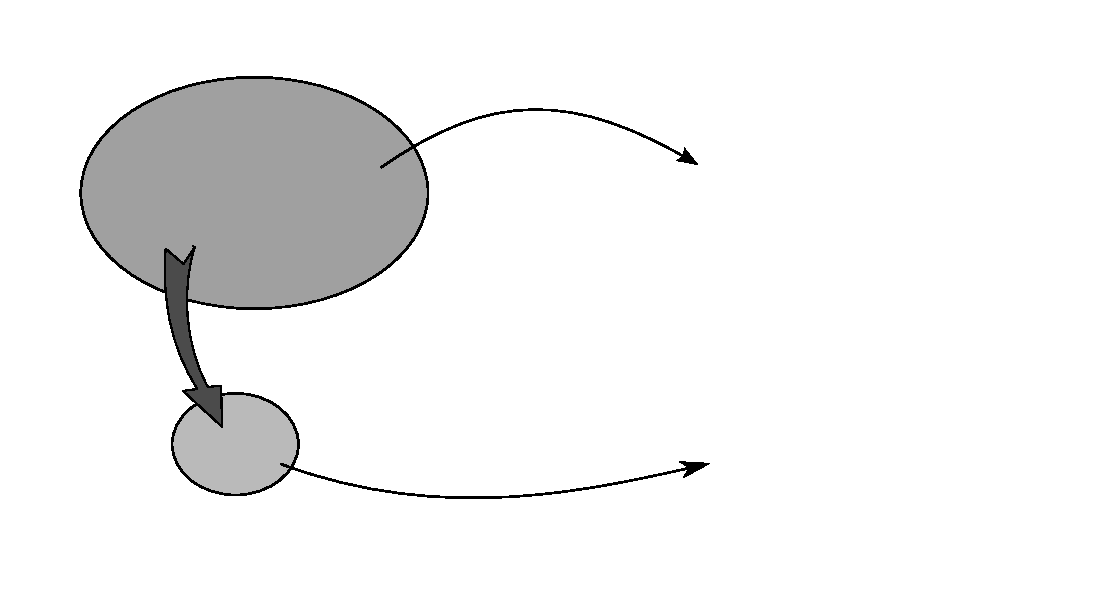
\includegraphics[width=10cm]{Dbes0104.eps}
		\put(-240,105){Poblaci\'o}
		\put(-260,135){$N$}
		\put(-150,135){$X$}
		\put(-110,125){$\mu_{X}, \sigma^2_{X}$}
		\put(-230,65){$n$}
		\put(-240,37){mostra}
		\put(-150,30){$Y$}
		\put(-110,25){$\mu_{Y}, \sigma^2_{Y}$}
	}
 \only<6>{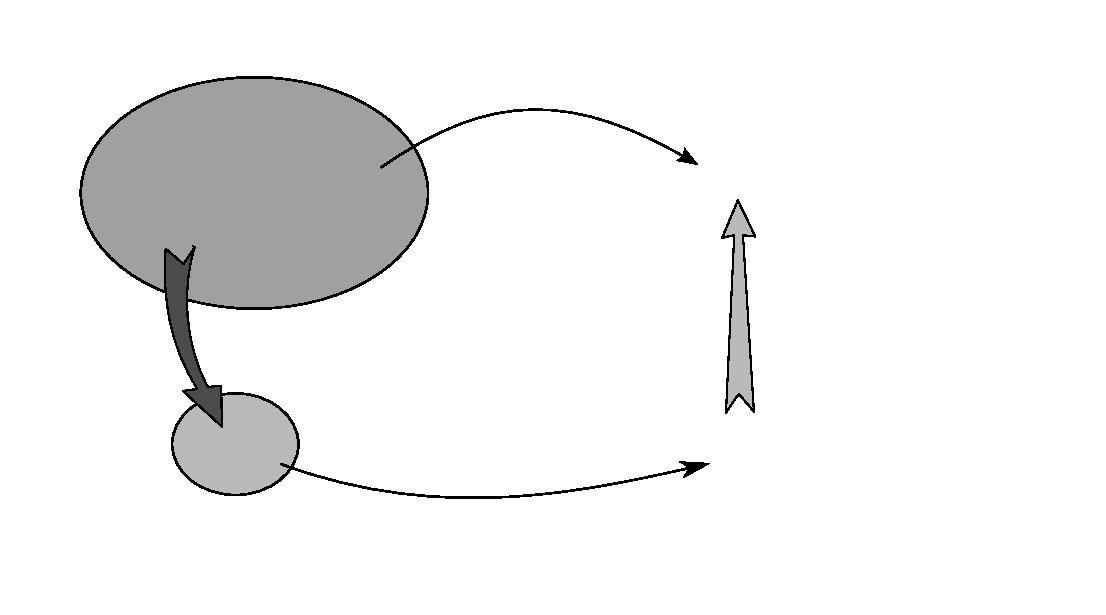
\includegraphics[width=10cm]{Dbes0105.eps}
		\put(-240,105){Poblaci\'o}
		\put(-260,135){$N$}
		\put(-150,135){$X$}
		\put(-110,125){$\mu_{X}, \sigma^2_{X}$}
		\put(-230,65){$n$}
		\put(-240,37){mostra}
		\put(-150,30){$Y$}
		\put(-110,25){$\mu_{Y}, \sigma^2_{Y}$}
		\put(-155,75){Probabilitat}
	}
 \only<7>{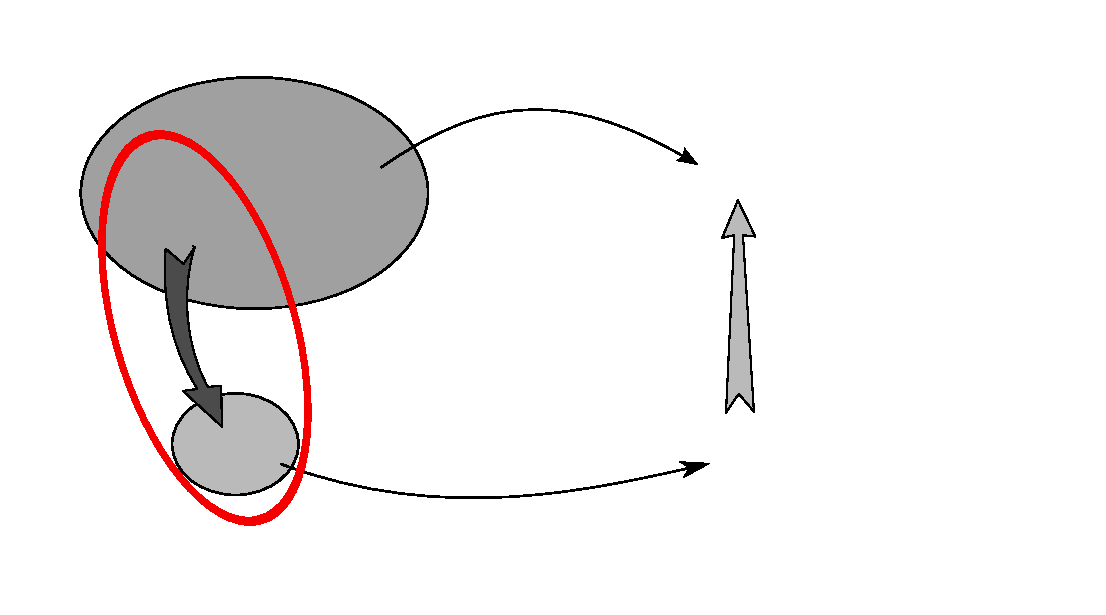
\includegraphics[width=10cm]{Dbes0106.eps}
		\put(-240,105){Poblaci\'o}
		\put(-260,135){$N$}
		\put(-150,135){$X$}
		\put(-110,125){$\mu_{X}, \sigma^2_{X}$}
		\put(-230,65){$n$}
		\put(-240,37){mostra}
		\put(-150,30){$Y$}
		\put(-110,25){$\mu_{Y}, \sigma^2_{Y}$}
		\put(-155,75){Probabilitat}
	}
 \only<8>{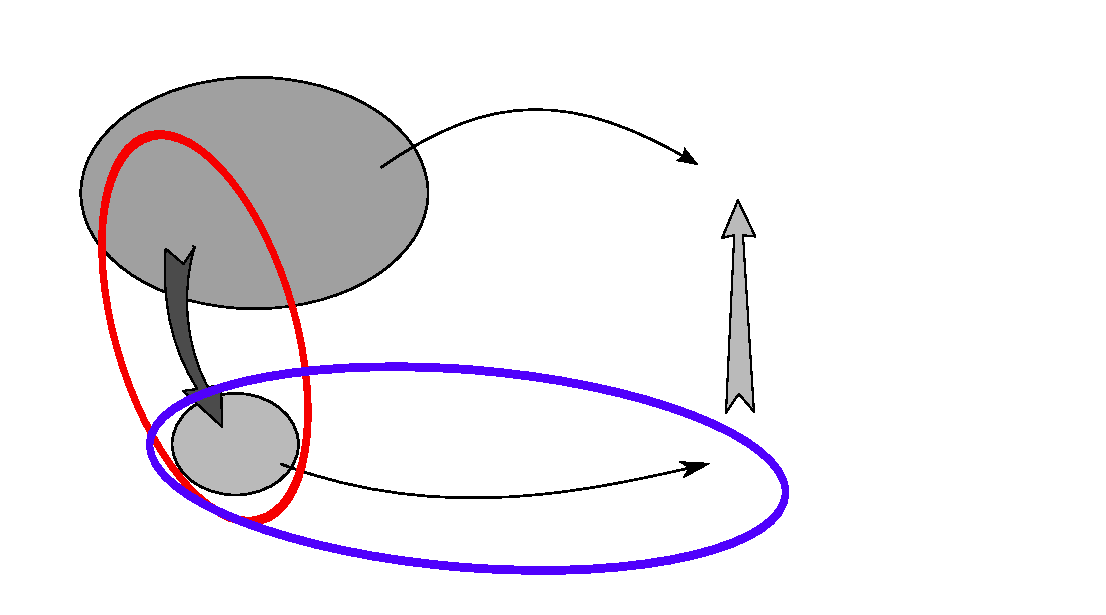
\includegraphics[width=10cm]{Dbes0107.eps}
		\put(-240,105){Poblaci\'o}
		\put(-260,135){$N$}
		\put(-150,135){$X$}
		\put(-110,125){$\mu_{X}, \sigma^2_{X}$}
		\put(-230,65){$n$}
		\put(-240,37){mostra}
		\put(-150,30){$Y$}
		\put(-110,25){$\mu_{Y}, \sigma^2_{Y}$}
		\put(-155,75){Probabilitat}
	}
 \only<9-10>{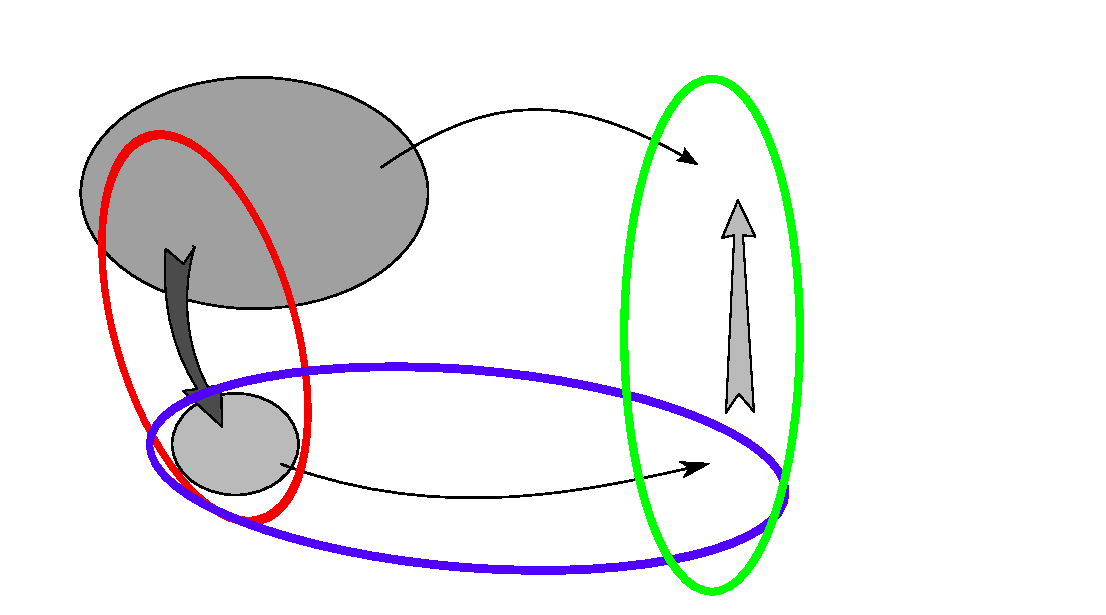
\includegraphics[width=10cm]{Dbes0108.eps}
		\put(-240,105){Poblaci\'o}
		\put(-260,135){$N$}
		\put(-150,135){$X$}
		\put(-110,125){$\mu_{X}, \sigma^2_{X}$}
		\put(-230,65){$n$}
		\put(-240,37){mostra}
		\put(-150,30){$Y$}
		\put(-110,25){$\mu_{Y}, \sigma^2_{Y}$}
		\put(-155,75){Probabilitat}
	}
\end{overlayarea}
\end{column}
\begin{column}{0.35\textwidth}
\begin{overlayarea}{0.95\textwidth}{0.65\textheight}
\only<2-6>{
	\begin{itemize} 
 	\item <2->$N$ tamany poblaci\'o
 	\item <3->$X$ Caracter\'{\i}stica 
 	\item <4->$n$ tamany mostra
 	\item <5->$Y$ Carac. mostral 
	\end{itemize}
	}
\only<7->{
	\begin{itemize} 
 	\item <7-9> \color{red}{\large Mostreig.}\color{black}
	\item[]
 	\item <8-> \color{blue}{\large Est. Descriptiva}\color{black}
	\item[]
 	\item <9-> \color{green}{\large Est. Inferencial}\color{black}
	\end{itemize}
	}
\end{overlayarea}
\end{column}
\end{columns}
}

\frame{\frametitle{Temari}
\begin{itemize}
\item Estad\'{\i}stica Descriptiva.
	\begin{itemize}
	\item [] Tema 1. An\`alisi exploratòria de dades.
	\item [] Tema 2. Distribucions estad\'{\i}stiques bidimensionals. 
	\item [] <2->\color{red}Examen parcial 15/03 \color{black}
	\item [] <2->\color{red}Entrega pràctiques 17/04 \color{black}
	\end{itemize}
\item Probabilitat.
	\begin{itemize}
	 \item [] Tema 3. Teoria de la probabilitat.
	 \item [] <3->\color{red}Examen parcial 03/04 \color{black}
	 \item [] <3->\color{red}Entrega problemes 03/04 \color{black}
	\end{itemize}
\item Estad\'{\i}stica Inferencial.
	\begin{itemize}
	\item [] Tema 4. Variables aleat\`ories discretes.
	\item [] Tema 5. Variables aleat\`ories continues.
	\item [] <4->\color{red}Examen parcial 17/05 \color{black}
	\item [] <4->\color{red}Entrega problemes 17/05 \color{black}
	\item [] Tema 6. Estimaci\'o de par\`ametres.
	\item [] Tema 7. Contrast d'hip\`otesi.
	\item [] <5->\color{red}Entrega problemes 07/06 \color{black}
	\end{itemize}
\end{itemize}
}

\end{document}